% !TEX root = exercises.tex

\exercisetitle{Exercise Sheet 3}

\begin{questions}
\question Find antiderivatives for the following functions:
\begin{parts}
\part $f(z) = \alpha + \beta(z-z_0)$,
\part $f(z) = (z-z_0)^n$,
\end{parts}
where $\alpha,\beta$ and $z_0 \in \C$ are constants and $n$ is an integer, $n \neq -1$.  Does $g(z)=(z-z_0)^{-1}$ have an antiderivative on $\C \backslash \set{z_0}$?  Question 6 on Exercise Sheet 2 may help here.  
\begin{answer}
\begin{enumerate}
\item[(a)] An antiderivative for $f$ on $\C$ is given by $F:\C \to \C$ where
\[
F(z) = \alpha z + \frac{1}{2} \beta z^2 - \beta z_0 z,
\]
since
\[
F'(z) = \alpha + ( \frac{1}{2} \beta ) (2z) - \beta z_0 = \alpha + \beta(z-z_0) = f(z)
\]
for all $z \in \C$.
\item[(b)] For $n \geq 0$ (respectively $n<-1$), and antiderivative for $f$ on $\C$ (respectively $\C \backslash \set{z_0}$) is given by $F$ where
\[
F(z) = \frac{1}{n+1} (z-z_0)^{n+1}.
\]
\end{enumerate}
The function $g$ does not have an antiderivative on $\C \backslash \set{0}$, since if it did, the Fundamental Theorem of Calculus would imply that
\[
\int_{\Gamma} g = 0
\]
where $\Gamma$ is the anticlockwise circular contour with centre $0$ and radius $1$.  We know from Exercise Sheet 2 that this integral has the value $2\pi i \neq 0$.
\end{answer}
\question Evaluate the following contour integrals:
\[
\int_{\mathcal{C}} z^3 \quad \text{ and } \quad \int_{\mathcal{C}} \frac{1}{z^2}
\]
along $\mathcal{C}$ where $\mathcal{C}$ is
\begin{parts}
\part any contour from $i$ to $-2$, and
\part any closed contour.
\end{parts}
For the second integral, you may assume that $\mathcal{C}$ does not contain $0$.
\begin{answer}
An antiderivative for $f(z) = z^3$ on $\C$ is given by the function $F$ with $F(z) = \frac{1}{4} z^4$.  Hence by the Fundamental Theorem of Calculus we have
\[
\int_{\mathcal{C}} z^3 = F(-2) - F(i) = \frac{1}{4} (-2)^4-\frac{1}{4} (i)^4 = \frac{15}{4}
\]
where $\mathcal{C}$ is any contour from $i$ to $-2$, and 
\[
\int_{\mathcal{C}} z^3 = 0
\]
when $\mathcal{C}$ is any closed contour.

Similarly $G(z) = \frac{-1}{z}$ is an antiderivative for $g(z) = \frac{1}{z}$ on $\C \backslash \set{0}$, and $\C \backslash \set{0}$ is a region in $\C$ (it is open and connected).  Hence by the Fundamental Theorem of Calculus we have
\[
\int_{\mathcal{C}} \frac{1}{z} = G(-2)-G(i) = \frac{-1}{-2} - \frac{-1}{i} = \frac{1}{2} -i
\]
for any contour $\mathcal{C}$ in $\C \backslash \set{0}$ from $i$ to $-2$, and
\[
\int_{\mathcal{C}} \frac{1}{z} =0
\]
for any closed contour $\mathcal{C}$ in $\C \backslash \set{0}$.

\end{answer}
\question Let $U$ be a region in $\C$ and let $f:U \to \C$ be holomorphic on $U$ with $f(z)$ real-valued for all $z \in U$.  Prove that $f$ is constant.
\begin{answer}
Write $f$ in the form
\[
f(x+iy)=u(x,y)+iv(x,y)
\]
where $u$ and $v$ are real-valued functions of two real variables.
If $f(z)$ is real valued then $v(x,y)=0$ on $U$, hence $\dfrac{\partial v }{\partial x} = \dfrac{\partial v}{\partial y}=0$ on $U$.

Since $f$ is holomorphic, $u$ and $v$ satisfy the Cauchy-Riemann equations, it follows that $\dfrac{\partial u}{\partial x} = \dfrac{\partial u}{\partial y}=0$ on $U$, hence
\[
f' = \frac{\partial u}{\partial x} + i \frac{\partial v}{\partial x} = 0
\]
on $U$. 

Since $U$ is connected, this implies that $f$ is constant by the Fundamental Theorem of Calculus.
\end{answer}


\question Find an upper estimate for
\[
\int_{\mathcal{C}} \frac{1}{1+z^4},
\]
where $\mathcal{C}$ is the upper semicircular contour from $R$ to $-R$ given by $\gamma:[0,\pi] \to \C$, $\gamma (t) = R \cos(t)+iR \sin (t)$.

\begin{answer}
We shall do this using the Estimation Lemma.  In order to apply the Lemma, we need to find $\ell{\Gamma}$ and an upper bound for $\abs{\frac{1}{1+z^4}}$ along $\mathcal{C}$.  Now, we know that
\[
\gamma '(t) = -R \sin(t) +i R \cos(t)
\]
with modulus
\[
\abs{\gamma'(t)} = \sqrt{ (-R\sin(t))^2+(R\cos(t))^2} = \sqrt{R^2(\sin^2(t)+\cos^2(t))} = R
\]
for all $t \in [0,\pi]$.  Hence the length of $\mathcal{C}$ is given by
\[
\ell(\mathcal{C})=\int_0^{\pi} \abs{\gamma'(t)} dt = \int_0^{\pi} R \ dt =\pi R.
\] 

Moreover, if $z$ lies in $\mathcal{C}$ then $z=\gamma(t)$ for some $t \in [0,\pi]$, hence
\[
\abs{z} = \abs{\gamma(t)} = \sqrt{(R\cos(t))^2+(R\sin(t))^2} = R.
\]
Using the backwards triangle inequality, for all $z \in \mathcal{C}$ we have
\[
\abs{1+z^4} \geq \abs{1-\abs{-z^4}} = \abs{1-R^4} = R^4-1
\]
(since $R>1$), and so
\[
\abs{\frac{1}{1+z^4}} \leq \frac{1}{R^4-1}
\]
whenever $z \in \mathcal{C}$.  Thus the Estimation Lemma tells us that
\[
\abs{\int_{\mathcal{C}} \frac{1}{1+z^4}} \leq \frac{1}{R^4-1} \cdot (\pi R) = \frac{\pi R}{R^4-1},
\]
so that $\pi R/(R^4-1)$ is an upper estimate for the integral $\int_{\mathcal{C}} 1/(1+z^4)$.


\end{answer}


\question Show that for all points $z$ on the circle $\set{z: \abs{z}=5}$ we have
\[
\abs{z-7} \leq 12 \quad \text{and}\quad \abs{\conj{z}+8} \geq 3,
\]
and use this to find an upper estimate for the integral
\[
\int_S \frac{z-7}{(\conj{z}+8)^2}\ dz
\]
where $S$ is the same circle oriented anticlockwise.

\begin{answer}
The first two inequalities can be shown using the triangle and backwards triangle inequalities respectively.  Using these, we have 
\[
\abs{\frac{z-7}{(\conj{z}+8)^2}} = \frac{\abs{z-7}}{\abs{\conj{z}+8}^2} \leq \frac{12}{3^2} = \frac{4}{3}
\]
for all $z \in S$.  The length of $S$ is $10\pi$, and so by the Estimation Lemma, we get the upper estimate
\[
\abs{
\int_S \frac{z-7}{(\conj{z}+8)^2}\ dz
}
\leq \frac{4}{3} \cdot 10\pi = \frac{40\pi}{3}.
\]
\end{answer}

\question Let $S_a$ be the anticlockwise square contour with corners at $\pm a(1+i),\pm a(1-i)$ where $a>0$.  Show that if $z \in S_a$ then
\[
\frac{1}{\abs{z}} \leq \frac{1}{a} \]
and hence
\[ \abs{ \int_{S_a} \frac{1}{z} dz } \leq 8,
\]
for all $a>0$.

\begin{answer}
Note that this square lies in the region outside the circle $\set{z:\C: \abs{z}=a}$.
\begin{center}
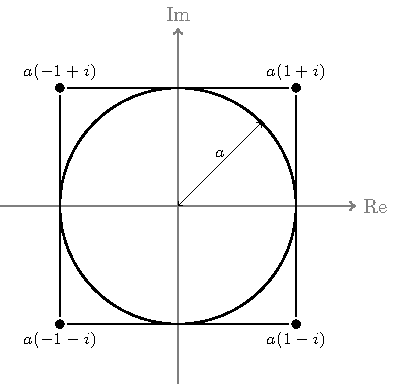
\includegraphics[scale=1]{squareandcircle}
\end{center}
Any point $z$ outside of this circle has modulus $\abs{z} \geq a$; in particular, this is true for any $z \in S_a$.  Hence for all such $z$, $\abs{\dfrac{1}{z}} \leq \dfrac{1}{a}$.

The length of each straight edge of $S_a$ is $2a$, and hence $\ell (S_a) = 8a$.  The Estimation Lemma then gives the required inequality.
\end{answer}

\question Prove each of the following:
\begin{parts}
\part For $z_0$ and $h$ in $\C$ we have $\displaystyle \int_{[z_0,z_0+h]} 1\ dz = h$.
\part For $f:U \to \C$ and $z_0 \in U$, $f(z_0) = \displaystyle \frac{1}{h} \int_{[z_1,z_1+h]} f(z_0)\ dz$.
\part If $\alpha$ is a complex number  and $M$ a fixed real number with $\abs{\alpha} \leq \epsilon M$ for all $\epsilon >0$ then $\alpha=0$.
\end{parts}
\begin{answer}
\begin{parts}
\part Using the parametrisation $\gamma:[0,1] \to \C$, $\gamma(t)=z_0+t(z_0+h-z_0) = z_0+th$, we have
$\gamma'(t)=h$ and $f(\gamma(t))=1$.  Hence
\[
\int_{[z_0,z_0+h]} 1dz = \int_0^1 f(\gamma(t)) \gamma '(t)\ dt = \int_0^1 1 (h) \ dt = h.
\]
Alternatively, using the antiderivative $F(z)=z$ for $f$, we have (by the Fundamental Theorem of Calculus)
\[
\int_{[z_0,z_0+h]} 1dz = F(z_0+h)-F(z_0)=z_0+h-z_0=h.
\]
\part Since $f(z_0)$ is a constant we have
\[
\frac{1}{h} \int_{[z_1,z_1+h]} f(z_0) dz = \frac{1}{h} f(z_0) \int_{[z_1,z_1+h]} 1 dz = \frac{1}{h} f(z_0) h = f(z_0)
\]
by the previous part.
\part Suppose that $\alpha \neq 0$.  Then $\abs{\alpha}>0$ (since for $z \in \C$ we have $\abs{z}=0$ if and only if $z=0$).  Setting $\epsilon = \abs{\alpha}/2M$ we have $\epsilon >0$, which implies that
\[
\abs{\alpha} \leq \epsilon M =  \frac{\abs{\alpha}}{2M} \cdot M = \frac{\abs{\alpha}}{2}.
\]
But this is only possible if $\abs{\alpha} =0$, a contradiction.  Hence $\abs{\alpha}=0$ and so $\alpha=0$.
\end{parts}
\end{answer}


\begin{comment}
\newpage


\question All of the proofs that have been done in lectures are examinable.  As some of these are quite long, you should be prepared to answer questions of the following format, where an outline of the proof is presented in the form of a series of statements.  For each numbered statement, provide a brief comment that explains or justifies it.  

\noindent{\bf Theorem (Cauchy's Theorem for a Triangle) } Let $\mathcal{R}$ be a simply connected region, $f$ a function that is holomorphic on $\mathcal{R}$ and let $T$ be a triangle in $\mathcal{R}$ with boundary $\partial T$.  Then
\[
\int_{\partial T} f =0.
\]
\medskip
{\bf Proof } 
There exists a nested sequence of triangles $\{ T_n \}$ such that
\[
\left( \frac{1}{4} \right)^n \left| \int_{\partial T} f \right| \leq \left| \int_{\partial T_n} f \right| \quad\text{ and }\quad \ell (\partial T_n ) = \left( \frac{1}{2} \right)^n \ell ( \partial T),
\]
and there is a point $z_0 \in \mathcal{R}$ with $z_0 \in T_n$ for all $n$.
\begin{enumerate}
\item[(1)] Given $\varepsilon >0$ there exists $\delta >0$ such that
\[
|z-z_0| < \delta \Longrightarrow \left| f(z)-f(z_0)-(z-z_0)f'(z_0) \right| \leq \varepsilon |z-z_0|
\]
\begin{answer}
Since $f$ is holomorphic on $\mathcal{R}$, $f$ is differentiable at $z_0$ and hence
\[
\lim_{z \to z_0} \frac{f(z)-f(z_0)}{z-z_0}
\]
exists and is equal to $f'(z_0)$.  

By the definition of a limit, given $\varepsilon>0$ there is $\delta >0$ such that
\begin{align*}
0< | z-z_0 | < \delta &\Rightarrow \left| \frac{f(z)-f(z_0)}{z-z_0}-f'(z_0) \right| < \varepsilon \\
& \Rightarrow \left| \frac{f(z)-f(z_0)-(z-z_0)f'(z_0)}{z-z_0} \right| < \varepsilon \\
& \Rightarrow \left| f(z)-f(z_0)-(z-z_0)f'(z_0) \right| < \varepsilon |z-z_0|.
\end{align*}
Finally, if $z=z_0$ then both sides of the final inequality are zero, which shows (1).
\end{answer}
\item[(2)] There exists $n$ such that $\ell ( \partial T_n) < \delta$ and $T_n \subset D(z_0;\delta)$.
\begin{answer}
Since $\ell ( \partial T)$ is fixed, we can choose $n$ large enough so that $\ell ( \partial T)/2^n < \delta$.  By the first (un-numbered) statement, for any such $n$ we have $\ell ( \partial T_n) < \delta$.

Since $z_0$ lies inside $T_n$, the distance from $z_0$ to any point on $\partial T_n$ is less than $\ell ( \partial T_n)$.
\end{answer}

\item[(3)]  For $z \in \partial T_n$
\[
\left| f(z)-f(z_0)-f'(z_0)(z-z_0) \right|< \epsilon \ell ( \partial T_n).
\]
\begin{answer}
By (2), for $z \in \partial T_n$ we have $|z-z_0| < \delta$, hence by (1), for all such $z$ we have
\[
\left| f(z)-f(z_0)-f'(z_0)(z-z_0) \right| \leq \varepsilon | z-z_0 | < \varepsilon \delta < \varepsilon \ell ( \partial T_n )
\]
the final inequality following from (2).
\end{answer}
\item[(4)] \hfil $\displaystyle \int_{\partial T_n} f(z)\ dz = \int_{\partial T_n} \left( f(z)-f(z_0)-f'(z_0)(z-z_0) \right)\ dz$\hfil
\begin{answer}
The (linear) function $z \mapsto f(z_0)+(z-z_0)f'(z_0)$ has an antiderivative on $\mathbb{C}$, and since $\partial T_n$ is a closed path,
\[
\int_{\partial T_n} f(z_0)+(z-z_0)f'(z_0)\ dz =0,
\]
so (4) follows from linearity of path integrals.
\end{answer}
\item[(5)]  \hfil $  \displaystyle \left| \int_{\partial T_n} f \right| \leq \varepsilon\ \left[\ell (\partial T_n ) \right]^2$ \hfil
\begin{answer}
The function $z \mapsto f(z) - f(z_0)-(z-z_0)f'(z_0)$ is bounded above on $\partial T_n$ by $ \varepsilon \ell ( \partial T_n )$ by (3), hence by the Estimation Lemma,
\[
\left| \int_{\partial T_n} f(z) - f(z_0)-(z-z_0)f'(z_0)\ dz \right| \leq \varepsilon \ell ( \partial T_n ) \cdot \ell ( \partial T_n ).
\]
Together with (4), this yields (5).
\end{answer}
\item[(6)] 
\hfil
$
 \displaystyle \left( \frac{1}{4} \right)^n \left| \int_{\partial T} f \right| \leq \left| \int_{\partial T_n} f \right| \leq \varepsilon\ \left[\ell (\partial T_n ) \right]^2 \leq \varepsilon \left(\frac{1}{4} \right)^n \left[ \ell ( \partial T) \right]^2.
$ \hfil
\begin{answer}
The first and last inequalities are given in the first (un-numbered) statement, the second was shown in (4).
\end{answer}
\item[(7)]\hfil $\displaystyle \int_{\partial T} f = 0 .$\hfil
\begin{answer}
By (6) we have
\[
\left| \int_{\partial T} f \right| \leq \varepsilon \left[ \ell ( \partial T ) \right]^2
\]
for all $\varepsilon >0$.  Since $\ell ( \partial T )$ is a constant, (7) follows.
\end{answer}
\end{enumerate}
\end{comment}



\end{questions}